\documentclass[a4paper,12pt]{article}

% Packages
\usepackage[utf8]{inputenc}
\usepackage{amsmath, amssymb}
\usepackage{graphicx}
\usepackage{hyperref}
\usepackage{geometry}
\usepackage{booktabs}
\usepackage{float}
\geometry{margin=1in}

% Title Page
\title{Merit Prize Challenge 2024/2025 \\ \vspace{0.5cm} \large Breast Cancer Dataset Analysis}
\author{Guilherme José & José Caldeira}
\date{November 2024}

\begin{document}

\maketitle
\tableofcontents
\newpage

% Sections
\section{Introduction}
\label{sec:introduction}
Overview of the challenge, dataset, objectives, and the methodology followed.

\subsection{Overview}
In this task we aim to develop a model that can accurately classify a patient with or without cancer based on available medical data. This is often used to support healthcare professionals in order to enhance efficiency and enabling doctors to help a larger number of patients effectively.
\subsection{Dataset description}
The dataset consists of \textbf{30 numerical variables} and \textbf{1 binary variable}, the target. Patients are classified as having a \textbf{benign tumor} or a \textbf{malignant tumor}, target variable is \textbf{0} or \textbf{1}, respectively. The dataset has \textbf{no missing values}.
\subsection{Logistic Regression}
Logistic regression is a machine learning method used to make binary classification. It differs from linear regression in the activation function and the loss function to update the weights. While in linear regression there is no activation function, logistic regression uses the sigmoid function:
\[ \sigma(z) = \frac{1}{1 + e^{-z}} \]


The expression of logistic regression is as it follows:
\[
\hat{y} = \sigma(\mathbf{w} \cdot \mathbf{x} + b) =\frac{1}{1 + e^{-(\mathbf{w} \cdot \mathbf{x} + b)}}
\]

\begin{itemize}
    \item \(\mathbf{w}\): The weight vector.
    \item \(\mathbf{x}\): The vector with each input variable
    \item \(b\): The bias term.
    \item \(\hat{y}\): The predicted probability of the positive class (\(y=1\)). 
\end{itemize}

To evaluate the model, we use cross validation as loss function:
\[
\text{Loss} = -\frac{1}{N} \sum_{i=1}^{N} \left[ y_i \log(\hat{y}_i) + (1-y_i) \log(1-\hat{y}_i) \right]
\]

\subsection{EM Clustering}
\subsection{RBF Network}
\textbf{Radial Basis Function} is a type of neural network that uses Radial Basis function as activation:
\[
\phi(x, c) = \exp\left(-\gamma \|x - c\|^2\right)
\]
\begin{itemize}
    \item \(\mathbf{x}\): The input vector.
    \item \(\mathbf{c}\): The centroid vector.
    \item \(\mathbf{\gamma}\): Parameter to control the width of the RBF. Also represented by \(\frac{1}{2\sigma^2}\).
\end{itemize}

RBF Networks have \textbf{3 layers}, one for the input, the middle layer, whose activation functino is RBF and the output layer. The  middle layer has k neurons, being \textbf{k} the \textbf{number of centroids} of the model. 

\section{Logistic Regression on the original data}
\label{sec:logistic-regression-original}
Logistic regression was applied to the raw dataset. These are the results:
\begin{itemize}
    \item \textbf{Confusion matrix}: 
    \[
    \begin{array}{|c|c|c|}
    \hline
    & \textbf{Predicted Positive} & \textbf{Predicted Negative} \\
    \hline
    \textbf{Actual Positive} & 107 & 1 \\
    \hline
    \textbf{Actual Negative} & 4 & 59 \\
    \hline
    \end{array}
    \]
    \item \textbf{Accuracy}: 97.1\%
    \item \textbf{Recall}: 99.1\%
    \item \textbf{Specificity}: 93.7\%
    
\end{itemize}

The accuracy score was excellent, this might be a confirmation that the dataset is complete and easily separable for this specific problem. Recall was even higher than accuracy, very close to 100\%. This is an important point to consider, as prioritizing an increase in recall should be given higher importance in the model’s objectives than increasing specificity.

\section{EM Clustering Analysis}
\label{sec:em-clustering}

\subsection{Clustering with Different \(k\) Values and Silhouette Evaluation}
EM clustering was applied to the original data with k values ranging from 2 to 10. Then we computed the silhouette metric for each of the models. These were the results:

\begin{figure}[H]
    \centering
    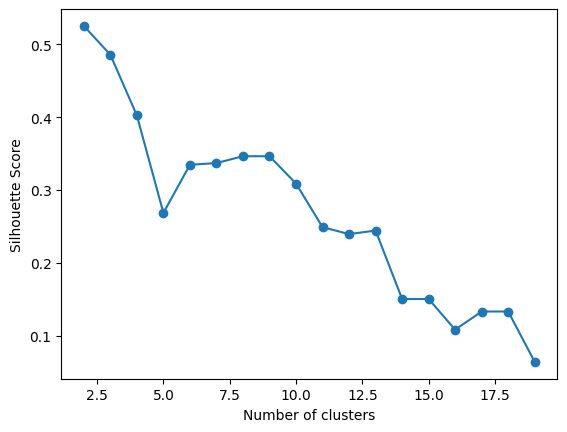
\includegraphics[width=0.8\textwidth]{imgs/silhouette.png}
    \caption{Silhoutte results across different k values.}
    \label{fig:silhouette}
\end{figure}


The results match perfectly with the nature of the problem. The more compact clusters were the ones that were binary, just like the nature of the classification tasks, which had a score of \textbf{0.63}. This confirms that the data can be easily separable, as previously mentioned in Section \ref{sec:logistic-regression-original}.

\subsection{Clustering Probabilities and Logistic Regression}
We used the previous clustering models and for each of the models, we mapped the dataset into clustering probabilities, meaning each observation is a vector of probabilities for each cluster.

Later, we used that mapped dataset to feed a logistic regression. These were the results:

\begin{figure}[H]
    \centering
    \begin{minipage}{0.48\textwidth}
        \centering
        \includegraphics[height=6cm]{imgs/accuracy_vs_k.png}  % Set a fixed height
        \caption{Accuracy results across different k values.}
        \label{fig:silhouette1}
    \end{minipage}
    \hfill
    \begin{minipage}{0.48\textwidth}
        \centering
        \includegraphics[height=6cm]{imgs/recall_vs_k.png}  % Set the same height
        \caption{Recall across different k values.}
        \label{fig:silhouette2}
    \end{minipage}
\end{figure}

The accuracy results show a slight increase from 2 to 3 in the x-axis (k values) and then decrease until k=8, after which it rises again. The first increase, even though silhouette is higher when k=2, 3 probability values might store more information than 2 and thus improve model accuracy. The decrease in accuracy is likely due to the poor silhouette score which makes the features (cluster probabilities) less informative. At the end there was a second increase in accuracy, this can be attributed to the increase in features outweight the poor silhouette scores.

The recall metric peaked when the accuracy was at its lowest, for \( k \in \{ 4, 6, 7, 8 \} \). This should be considered when choosing and evaluating models.



\section{RBF Network Training}
\label{sec:rbf-network}
Training of the RBF network using the clustering with optimal \(k\).

\section{Discussion}
\label{sec:discussion}
Key findings, correlations, and overall insights from the analysis.

\section{Conclusion}
\label{sec:conclusion}
Summary of the challenge, results, and future directions.

% References Section
\section*{References}
\label{sec:references}

\end{document}